\section{Observer}
\begin{frame}{Observer}
	\begin{block}{Was ist ein Observer?}<+->
		Ein Observer überwacht andere Objekte
	\end{block}
	\begin{block}{Wann ist ein Observer besonders sinnvoll?}<+->
		Um unabhänig vom Rest zu arbeiten
	\end{block}
	\begin{block}{Warum haben wir einen Observer eingesetzt?}<+->
		Wir haben ausgelagerte Threads per Observer eingebunden
	\end{block}
\end{frame}
\subsection{Observer OOD}
\begin{frame}{Observer OOD}
	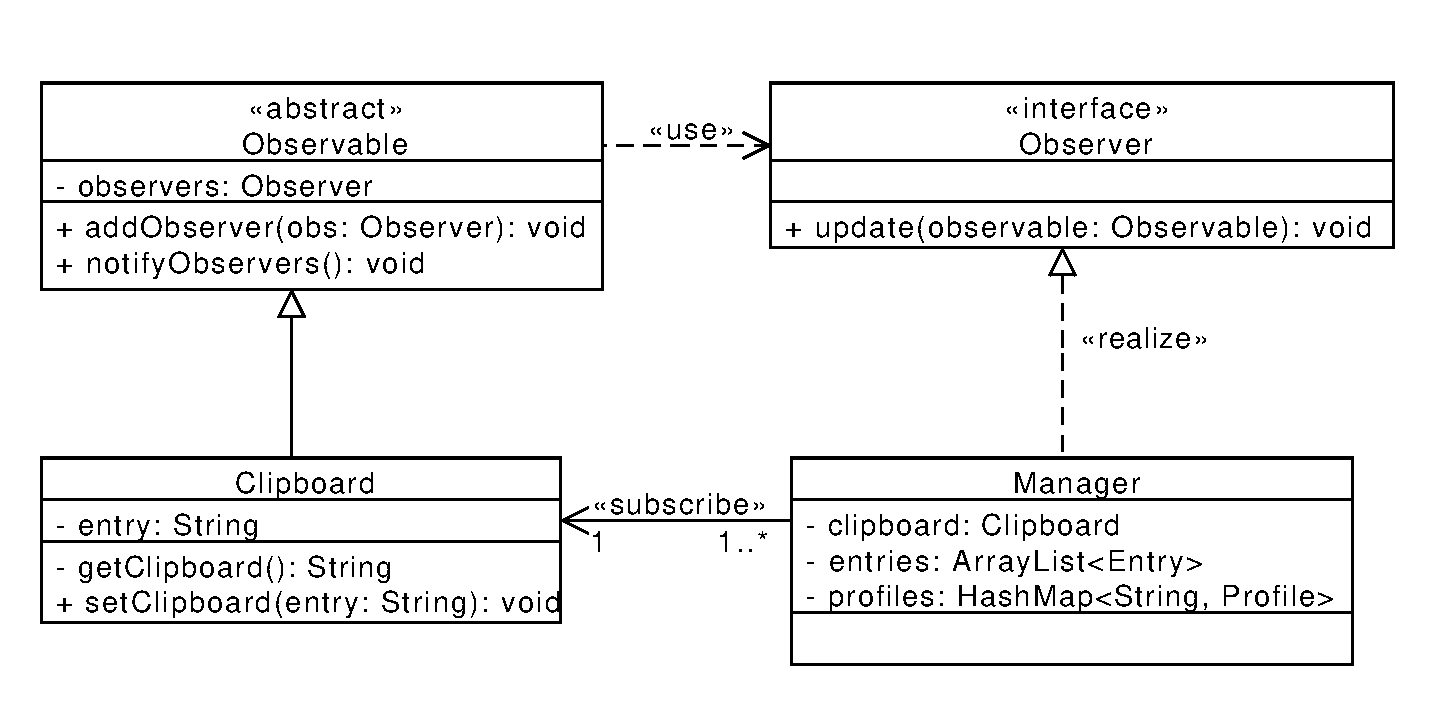
\includegraphics[width=\dimexpr\textwidth]{observerEx.pdf}
\end{frame}
